\chapter[The comparator]{The comparator: what beating Jev can and cannot mean}
\label{ch:comparator}

The product claim is comparative: faster, smaller and cheaper than Jev. A
comparative claim is only as good as its comparator, so this chapter states
what can be measured from this machine, what can only be cited, and which
comparisons the evidence does not support at all. The distinction is not
rhetorical. A committee that cannot tell a measured number from a vendor's
number cannot audit either.

\section{What Jev publishes, and what a third party measured}

TypeSafe's launch post is specific about three things and silent about the
rest \citep{typesafe2026jev}. It states a price of \$0.042 per million input
tokens with output billed at zero; an end-to-end response time of 70--500\,ms;
and a sampling mechanism that is \emph{parallel} --- ``generates all outputs in
a single query'' --- with possible outputs ``defined in advance'', so that the
model cannot emit a value outside the declared set. That is the same mechanism
this thesis measures in its \emph{score} arm. The post publishes no parameter
count, no architecture and no weights, and no reproducible per-task harness; its 193.6$\times$
and 444.6$\times$ headline figures are vendor-run workflow evaluations against
a reference answer built from two frontier models, which the post itself calls
``on the higher end of real world gains''.

The task-level numbers the suite pre-registered against are third-party. \citet{ayautomate2026jev}
ran Jev 1.13 through OpenRouter's decisions endpoint against 791 labeled
decisions, giving every system the same instruction and the same label list.
On Banking77 77-way intent routing --- 231 items, three per intent --- Jev
scored \textbf{78.8\%} (95\% Wilson interval 73.1--83.6), with a median latency
of 0.33\,s and a billed cost of \$0.0400 per thousand decisions, at 952 billed
input tokens per 77-way decision. On the same items it was not distinguishable
from GPT-5.4 nano (78.4\%) and was 5.2 points behind GPT-5.6 Terra, a gap their
paired test calls real.

That is the number the suite pre-registered against, and the comparison below
uses it. It is not the strongest public Jev number: a separate reproducible run
scores the full test set with retrieved examples and reports 92.40\%, and
\S\ref{sec:jev-strongest} states what that does to the verdict. The
protocol-matched test of that run is \S\ref{sec:jev-matched}.

\section{The falsification criterion, stated before the results}

The claim under test is: \emph{a byte-level decider that scores a finite
candidate set is faster, smaller and cheaper per decision than a Jev-style
service at equal accuracy.} It is falsified if any of the following holds.

\begin{enumerate}
  \item \textbf{Mechanism.} Generation matches or beats exhaustive scoring in
        accuracy at a matched training budget, on the same encoder and rows.
        Then the \emph{score} mechanism buys nothing and the architectural
        argument collapses, whatever the price.
  \item \textbf{Accuracy at 77-way.} The shipped rung's 77-way accuracy sits far
        below the cited 78.8\% (the pre-registered comparator; the stronger
        92.40\% run is audited in \S\ref{sec:jev-strongest}). Then the ``at equal accuracy'' clause is not
        met, and no speed or cost advantage can be claimed to compensate for
        it. This criterion is stated first among the empirical ones because it
        is the one this thesis is most likely to fail.
  \item \textbf{Cost.} The break-even GPU rate --- the hourly price at which
        1,000 local decisions cost what Jev charges for the same payload ---
        falls below the rate of the hardware the model actually runs on. Then
        local scoring is not cheaper.
  \item \textbf{Speed.} Measured per-decision latency exceeds Jev's published
        70--500\,ms band or the third-party 0.33\,s median on comparable
        payloads. Then the speed claim is false even before hardware is
        considered.
  \item \textbf{Size.} The claim is \emph{unfalsifiable as stated}, because
        neither TypeSafe nor the third-party run publishes a parameter count.
        A size comparison cannot be won; this thesis reports its own artifact
        size and records the axis as not comparable.
\end{enumerate}

\section{Mechanism: decode versus score}

Table~\ref{tab:comparator} holds the encoder, the initialisation, the rows, the
order, the number of steps, the batch size, the learning rate and the seed
fixed, and varies only the interface. The \emph{score} arm evaluates all $K$
candidates in one pass and cannot produce an out-of-bank label. The
\emph{decode} arm fine-tunes the same encoder as a conditional byte model and
fills the label's byte slots iteratively, then matches the emitted string
against the bank; it can produce an out-of-bank label, and that rate is
reported rather than hidden.

The choice of mask-fill rather than causal autoregression is deliberate and
costly, and it is stated here rather than buried: a causal decoder would be a
different set of weights, so comparing it with the scorer would confound
``generation'' with ``a differently trained model''. Mask-fill keeps the
weights and the data identical and changes only the loss and the interface.
The price of that choice is that mask-fill needs one pass per label length, so
its latency is a \emph{lower bound} on what an autoregressive decoder of the
same label length would pay --- which biases the comparison \emph{in favour of}
decoding, not against it.

\begin{table}[htbp]
\centering
\footnotesize
\caption{Decode versus score with everything else fixed: same encoder, same
initialisation, same rows in the same order, same steps, batch, learning rate
and seed. \emph{Score} evaluates every candidate in one pass and cannot emit an
out-of-bank label; \emph{decode} fills the label's byte slots iteratively and is
matched against the bank, so it can. Latency is batch-1 wall clock on CPU over
the same test rows, and therefore a lower bound on what an autoregressive
decoder of the same label length would cost. GPU seconds per 1,000 decisions
come from $1000\times p_{50}$ and are CPU seconds here, so they overstate an
accelerator. The last column is the GPU rate at which 1,000 local decisions
cost what Jev charges for that task's billed payload at \$0.042/MTok; it is rate-free
because no price for this machine is recorded anywhere in the repository. Read
from \texttt{results/decode\_vs\_score/*.json}.}
\label{tab:comparator}
\setlength{\tabcolsep}{4pt}
\begin{tabular}{lrrrrrrrrr}
\toprule
Task & $K$ & Seats & Score acc. & Decode acc. & Invalid & $p_{50}$ score & $p_{50}$ decode & GPU s & break-even \\
 & & & & & rate & (ms) & (ms) & per 1k & \$/GPU-h \\
\midrule
ag-news & 4 & 3 & 0.5011 & 0.1444 & 0.58 & 15.1 & 68.6 & 15.1 & 3.6 \\
banking77 & 77 & 3 & 0.8430 & 0.0000 & 1.00 & 28.2 & 248.4 & 28.2 & 5.1 \\

\bottomrule
\end{tabular}
\end{table}


On the 4-way task, across \CmpNewsSeeds{} seeds, scoring reaches
\CmpNewsScore{} against \CmpNewsDecode{} for decoding, with \CmpNewsInvalid{}
of decoded outputs outside the bank. On the 77-way task the same comparison
runs over \CmpBankSeeds{} seeds at $K=\CmpBankK$ and much longer labels:
scoring reaches \CmpBankScore{} against \CmpBankDecode{}, with
\CmpBankInvalid{} of decoded labels unusable. Both arms are the same
2,411,200-parameter network and the same 9.7\,MB on disk in every row; the only
difference is how the answer is produced.

The mechanism result is therefore not marginal: at this size and budget,
exhaustive scoring is more accurate, several times faster, and cannot leave the
answer space, while generation drifts outside it one time in two on 4-way and
more often as $K$ grows and the label gets longer. That is the finding the
architecture claim rests on, and it is narrow in a way worth stating plainly:
it says nothing about what a larger generative model with a hundred times this
compute would do. What it says is that the mechanism's advantage is not
purchased with parameters --- the only version of the claim a 2.4M-parameter
checkpoint is entitled to make.

\section{The 77-way number, side by side}

Table~\ref{tab:jev77} is the comparison the product claim actually needs, and
the one this thesis is least able to win. It is assembled from two different
experiments: fine-tunes of this project's checkpoint on 1,600 and 8,000
Banking77 training rows drawn evenly across all 77 labels, and a third party's
zero-shot calls to a hosted model on 231 test items, with labels supplied as the
option list. The rows are not the same rows, the hardware is not the same
hardware, and one system is measured by its authors while the other is measured
by a stranger. Every cell carries its evidence class for exactly that reason.

\paragraph{A correction, recorded rather than quietly replaced.}
An earlier version of this table used a loader's sorted prefix. Banking77 ships
label-sorted: forty consecutive rows share a label, so a loader that takes the
first $n$ rows returns a prefix of a few classes, not a sample of the task. The
number that loader produced was not a 77-way accuracy, and it is quarantined
under \texttt{results/decode\_vs\_score/\_sortedprefix\_bug/} rather than
quoted. The replacement draws class-balanced subsets (\texttt{--stratify}),
fixed by a split seed so that every training seed sees exactly the same rows.
The corrected 8,000-row number is \CmpBankScorePct\%, with a different row
budget from the decode arm; the 1,600-row score is reported separately in
Table~\ref{tab:rows}.

\begin{table}[htbp]
\centering
\footnotesize
\caption{Banking77 77-way, the public task-level comparison with a third-party Jev run.
\emph{Measured} cells come from \texttt{scripts/decode\_vs\_score.py} on this
machine, over a class-balanced draw of all seventy-seven labels; \emph{cited}
cells come from a third party's run of a hosted API \citep{ayautomate2026jev}.
The score row is the 8{,}000-row fine-tune; the decode row is the 1{,}600-row
arm, so the row budgets differ within this table as well as across systems. The
two systems were never evaluated on the same rows or the same hardware, so a
difference of a few points would prove nothing and a large difference would.}
\label{tab:jev77}
\setlength{\tabcolsep}{4pt}
\begin{tabular}{p{0.20\linewidth}rrrrp{0.16\linewidth}}
\toprule
System & Accuracy & $p_{50}$ latency & Cost per 1k & Params & Evidence \\
\midrule
Azurite, score & \CmpBankScore & \CmpBankLatScore\,ms & \CmpBankGpuSec{} GPU-s & 2.41M & measured \\
Azurite, decode & \CmpBankDecode & \CmpBankLatDecode\,ms & \CmpBankGpuSec{} GPU-s & 2.41M & measured \\
Jev 1.13 & 78.8\% (73.1--83.6) & 330\,ms & \$0.0400 & not published & cited \\
GPT-5.4 nano & 78.4\% (72.6--83.2) & 1,150\,ms & \$0.2049 & not published & cited \\
\bottomrule
\end{tabular}
\end{table}

Read plainly, the table says two things. First, on accuracy this project has a
number on the 77-way task where a public Jev number exists: \CmpBankScorePct\%
(95\% Wilson interval \CmpBankScoreLo--\CmpBankScoreHi) over \CmpBankRows{}
held-out rows, against the cited 78.8\% (73.1--83.6); the measured interval
\CmpBankVerdict. The hedging is deliberate: those two intervals come from
different samples, of different sizes, drawn by different harnesses on
different hardware, so an overlap is not proof of parity and a small
non-overlap is not proof of superiority. A paired McNemar test on the same 231
items is the experiment that would settle it, and it is not this one. Second,
on the axes the product claim leans on, the same checkpoint is competitive:
\CmpBankLatScore\,ms against a 330\,ms cited median, and \CmpBankGpuSec{}
GPU-seconds per thousand decisions against a billed \$0.0400.

Both statements belong in the thesis, and neither cancels the other. Accuracy
is the load-bearing axis, and the honest reading of the table is not that the
mechanism failed --- the decode arm failed far harder, at \CmpBankDecodePct\%
with \CmpBankInvalid{} of its labels unusable --- but that a 2.41M-parameter
byte model is only as good as the data it is shown. This is the 2.41M
mechanism-and-cost comparison, not the project's best accuracy: the 14.4M suite
reaches \SuiteSmallBank\% on Banking77 under the final recipe, and that row is
reported in \S\ref{sec:suite}. The two are different checkpoints, recipes and
test draws and are not interchangeable.
Section~\ref{sec:rows-and-rung} measures that lever directly: the same
checkpoint given five times the fine-tune rows is a different system. The 84.3\%
row is the 8,000-row arm; the 1,600-row arm is 72.3\%, and the two must not be
read as a single budget.

\subsection{The strongest public Jev run, and what it does to the claim}
\label{sec:jev-strongest}

The 78.8\% cell above is the pre-registered comparator, not the strongest public
Jev number. \citet{smith2026jevbanking} ran Jev 1.13 on all 3,080 official
Banking77 test rows, supplying 24 retrieved labelled training examples and
definitions of all 77 categories with each request; Jev scored \textbf{92.40\%}
(95\% Wilson 91.41--93.29; 2,846 correct) at \$0.1421 per thousand decisions.
That is above the 113.47M suite's \SuiteLargeBank\% on its 2,000-row stratified
draw and above this 2.41M arm's \CmpBankScorePct\%. The input regimes differ:
the Jev run retrieves examples per request and scores the full official test
set, while the suite fine-tunes on 4,000 rows and scores a stratified 2,000-row
draw. The difference is large enough to change the verdict. Against the
pre-registered 78.8\% comparator the Banking77 cell is a clear win; against the
strongest public Jev run it is a loss. Both statements are reported, and the
weaker comparator is not used to claim a benchmark victory.

The audit also explains why the two Jev numbers coexist. The 78.8\% run is
zero-shot with an option list; the 92.40\% run supplies labelled examples and
category definitions, the regime in which a decision model is actually deployed.
A fair head-to-head gives both systems the same rows and the same examples on
all 3,080 rows. That experiment is reported in \S\ref{sec:jev-matched}; it
returns a negative verdict for the mean-pool head. \S\ref{sec:jev-query} then
tests the pooling diagnosis with a separately pre-registered query-anchored
head. That head recovers the example context but does not meet the P0 bar
either.

\subsection{The protocol-matched test, and its verdict}
\label{sec:jev-matched}

The comparison above is a comparison of two protocols. It can say that 92.40\%
is higher than \SuiteLargeBank\%, but not that the same system, on the same rows
and with the same information, would be higher. This subsection reports the
test that removes that ambiguity.

The protocol was written and hashed before any Azurite forward pass on the full
set (\texttt{results/jev\_matched/PRE\_REGISTRATION.md}, SHA-256
\texttt{\JevMatchPreregSha}). It fixes all \JevMatchN{} official test rows in
the public run's order; the exact 24 retrieved labelled examples that run
supplied for each row, in the same order; the same gold labels and the same Jev
correctness vector; Azurite's existing 113.47M full-bank head at a
5{,}120-byte window; top-1 accuracy with a 95\% Wilson interval; a $-2.0$
point non-inferiority margin on the paired bootstrap; and superiority only if
the point estimate is at least Jev's and exact McNemar $p<0.05$. Three arms
were fixed: message only at 1{,}024 bytes (A0, the row-set diagnostic), the 24
examples truncated to 1{,}024 bytes (A2, the length diagnostic), and the full
24 examples at 5{,}120 bytes (A1, primary). The 77 category definitions are not
supplied to Azurite: its information budget is strictly smaller than Jev's, and
that asymmetry is stated in the pre-registration so a win could not be
attributed to extra information.

\begin{table}[htbp]
\centering
\footnotesize
\caption{The protocol-matched Banking77 comparison. All 3{,}080 official test
rows, in the public run's order; the same 24 retrieved labelled examples per row,
in the same order; gold labels from the same frozen prediction file. Azurite is
not given the 77 category definitions, so its information budget is strictly
smaller than Jev's. The primary arm was fixed at A1 with a $-2.0$ point
non-inferiority margin before any forward pass. Wilson intervals are 95\%;
McNemar is exact and two-sided; the paired bootstrap lower bound is the 5th
percentile of 10{,}000 resamples, seed 0. Read from
\texttt{results/jev\_matched/summary.json}; the pre-registration hash is
\texttt{\JevMatchPreregSha} and the evaluator-only amendment is
\texttt{\JevMatchAmendmentSha}.}
\label{tab:jev-matched}
\setlength{\tabcolsep}{1.5pt}
\begin{tabular}{@{}lrrrrrrrrr@{}}
\toprule
Arm & Ex. & Window & Eff. & $n$ & Correct & Acc. & 95\% Wilson & $\Delta$ vs Jev & McNemar $p$ \\
 & & (bytes) & ex. & & & (\%) & & (pp) & \\
\midrule
A0 message only & 0 & 1{,}024 & 0.0 & 3{,}080 & 2{,}722 & 88.38 & 87.20--89.46 & $-$4.03 & $8.49\times10^{-12}$ \\
A2 24 examples, truncated & 24 & 1{,}024 & 12.2 & 3{,}080 & 1{,}793 & 58.21 & 56.46--59.94 & $-$34.19 & $1.21\times10^{-237}$ \\
A1 24 examples (primary) & 24 & 5{,}120 & 24.0 & 3{,}080 & 691 & 22.44 & 21.00--23.94 & $-$69.97 & $<10^{-300}$ \\
Jev 1.13, cited & 24 & vendor & 24 & 3{,}080 & 2{,}846 & 92.40 & 91.41--93.29 & --- & --- \\
\bottomrule
\end{tabular}
\end{table}


The result is not close. A0 reaches \JevMatchPctNoEx\%
(\JevMatchNoExLo--\JevMatchNoExHi), \JevMatchGapNoEx{} points below Jev; A2
reaches \JevMatchPctATwo\%; A1 reaches \JevMatchPctAOne\%
(\JevMatchAOneLo--\JevMatchAOneHi). The pre-registered verdict is that
\textbf{\JevMatchVerdict}: the paired bootstrap lower bound is
\JevMatchLowerAOne{} points, the exact McNemar test has $p\JevMatchPAOne$, and
A1 is neither non-inferior nor superior.

Two things follow, and they are different. First, the row-set confound is dead:
A0, on all 3{,}080 official rows with no examples, is \JevMatchGapPrimary{}
points below Jev and within a fraction of a point of the 2{,}000-row suite
value (\SuiteLargeBank\%). The earlier 88.45\% versus 92.40\%
gap was not a sampling artifact. Second, the examples do not help this
checkpoint; they destroy it. Accuracy falls monotonically as the context grows,
from \JevMatchPctNoEx\% at zero to \JevMatchPctATwo\% at a
mean of \JevMatchEffATwo{} complete examples to \JevMatchPctAOne\% at all
\JevMatchEffAOne. That pattern is consistent with pooling dilution, but A1 changes two things at
once and only A2 isolates one of them. A2 holds the window at the head's native
1{,}024 bytes and still falls to \JevMatchPctATwo\% at a mean of
\JevMatchEffATwo{} complete examples, so examples alone cost about 30 points
inside the trained length. A1 extends the same serialization to 5{,}120 bytes,
beyond the 1{,}024 positions the head was trained on; RoPE grows its table but
not its training distribution. The further fall to \JevMatchPctAOne\% is
therefore a joint example-and-length transfer failure, not an examples-only
effect. The mechanism is still visible: \texttt{AzuriteDual.\_pool} mean-pools
every non-padding token, so a multi-example context reduces the customer message
to a few percent of the pooled vector, and the head was trained only on
message-only contexts. Prediction concentration points the same way: A1 still
uses \JevMatchDistinctAOne{} of the 77 labels, but its most frequent label takes
\JevMatchTopAOne\% of rows and its three most frequent take
\JevMatchTopThreeAOne\%, against \JevMatchTopNoEx\% for the most frequent label
in A0. The examples are not being read as references; they shift the pooled
vector toward whichever intents dominate the retrieved set. The clean causal
claim is narrower than ``the examples are useless'': the head cannot use them
without losing accuracy even at its native window, and extending the window
makes the loss worse.

This is a negative result about the mean-pool head, not a ceiling for the
architecture. No model in the suite was trained to read retrieved examples; the
suite head is a zero-shot-context fine-tune. The pre-registered failure rule
named the intervention the evidence selected --- a query-anchored,
retrieval-augmented head, with a learned attention pool over the token sequence,
fine-tuned on the same 4{,}000 rows at the native 1{,}024-byte window with the
same BM25 examples that fit. That intervention was run under its own hashed
pre-registration and is reported in \S\ref{sec:jev-query}; it changes the
pooling architecture, so the mean-pool result above remains its control. The recorded evidence, the amendment that fixed an
evaluator-only grad-context bug (the A0 and A1 per-example files are
byte-identical under both evaluators), and the full per-example records are
under \texttt{results/jev\_matched/}; \texttt{VERDICT.md} is generated from
\texttt{summary.json}, not typed.

\subsection{The query-anchored head: testing the pooling diagnosis}
\label{sec:jev-query}

The preceding subsection identifies mean pooling as the mechanism but does not
test it. A second protocol, hashed before any training step
(\texttt{results/jev\_query/}\allowbreak
\texttt{PRE\_REGISTRATION.md}, SHA-256 \texttt{\QueryPrereg}), fixes the
architecture, the 4{,}000-row draw, the BM25
retrieval, the 1{,}020-byte complete-example packing, the optimisation recipe,
the four evaluation arms and the P0 rule. Two evaluator-only amendments are
recorded: one fixes candidate-embedding dispatch, the other manifest path
resolution. Neither changes a hypothesis, arm, row, context, metric or the
decision rule. The head is \texttt{QueryDual}: the same byte encoder,
initialised from the 113.47M checkpoint, with a masked attention pool over the
context whose query is a linear map of the mean-pooled customer message, and
the same candidate projection as the old head.

Table~\ref{tab:query-head} reports the four arms. The primary arm reaches
\QueryPctQueryTwo\% (95\% Wilson \QueryLoQueryTwo--\QueryHiQueryTwo),
\QueryDiffAbs{} points below Jev's
\QueryJevPct\%. The exact McNemar test against the public per-example vector
gives $\QueryPValueText$, the paired bootstrap lower bound is
\QueryLowerPrimary{} points, and the arm is not non-inferior at the
pre-registered $-2.0$-point margin. The verdict is \textbf{\QueryVerdict}: the
bar is not met, and the interval does not contain it.

The controls identify what changed. The old head on the identical contexts
reaches \QueryPctOldTwo\%, so the query pool is worth \QueryMechGain{} points
(exact McNemar $\QueryMechPText$, bootstrap lower \QueryMechLower). That is the
pooling diagnosis confirmed: the examples were never unreadable, they were
averaged away. The query head without examples reaches \QueryPctQueryZero\%, but
that arm is out of distribution --- the head was trained only on contexts that
contain examples --- so it is a control for the example context, not a
fair no-example baseline; it shows the head learned to use the examples
(\QueryVsZeroGain{} points). Yet the primary arm is only
\QueryVsOldZeroGain{} points above the old head's no-example arm
(\QueryPctOldZero\%). At this budget the retrieved examples recover what mean
pooling destroyed and buy almost nothing beyond the message itself.
Figure~\ref{fig:pooling} places the message-only, native and packed-5{,}120
settings side by side for both heads.

\paragraph{Contamination check.} The frozen 24-example record is not
test-clean. Under normalised text (NFKC, case-folding, punctuation collapsed),
\ContamSupportMatches{} of the \ContamSupportOriginal{} support messages are
official test rows (\ContamSupportExact{} exact; \ContamSupportShare\% of the
bank), and all \ContamSupportSameLabel{} carry the same gold label. They occur
in the frozen example sets of \ContamEvalRows{} of the \ContamCleanN{} rows
(\ContamEvalShare\%), as \ContamInstances{} instances: \ContamSelf{}
self-retrievals and \ContamCross{} cross-row retrievals. \ContamCrossRows{}
rows retrieve at least one cross-row test message, and \ContamCrossOnlyRows{} do so
without also retrieving their own message. \ContamSameLabel{} instances carry
the row's gold label and \ContamDiffLabel{} a different label, so this is a
content leak, not a label leak. The contamination is not uniform: the other
\ContamUnaffectedN{} rows retrieve no test text, so \QueryPctQueryTwo\% is a
mixture rather than a constant shift on every row.

The original product path over the 9{,}993-row bank is not an independent
corroboration of that arm: it produced the same prediction on all
\ContamCleanN{} rows and the same context digest on
\ContamProductFrozenSameContext{} of them. The wheel now ships the decontaminated
bank (\ContamSupportClean{} rows): removing all \ContamSupportMatches{} test
messages from the support bank and re-running the same BM25 path changes
\ContamCleanContextChanged{} contexts and \ContamCleanPredSame{} predictions; it
scores \ContamCleanCorrect/\ContamCleanN
= \ContamCleanAcc\% (95\% Wilson \ContamCleanLo--\ContamCleanHi), a change of
\ContamCleanDiff{} points (\ContamCleanWins{} wins, \ContamCleanLosses{} loss;
exact McNemar \ContamCleanPText). The \ContamUnaffectedN{} rows that never
retrieved a test message score \ContamUnaffectedCorrect/\ContamUnaffectedN =
\ContamUnaffectedAcc\% (95\% Wilson \ContamUnaffectedLo--\ContamUnaffectedHi).
The gap to Jev therefore survives decontamination: \QueryPctQueryTwo\% remains a
valid measurement of the frozen-example arm, but it is not a clean held-out
estimate. Excluding only the 25 rows that retrieve their own text is not
sufficient: 230 rows still retrieve another test row. The genuinely unaffected
subset is the \ContamUnaffectedN-row result above, and the full decontaminated
rerun is \ContamCleanAcc\%.

The remaining gap is therefore an information gap, not a pooling gap. The
primary arm fits \QueryEff{} complete examples on average (range
\QueryEffMin--\QueryEffMax) into 1{,}020 bytes, and it is given no category
definitions. The public Jev run supplies all 24 examples and definitions of all
77 categories in a much longer context. The first next lever --- a 5{,}120-byte joint fine-tune with all 24 examples ---
was run under its own hashed pre-registration and amendment and is reported in
\S\ref{sec:jev-len5120}; it cost \LenHeadHours{} GPU-hours. It tests whether the
example budget alone accounts for the gap; 5{,}120 bytes holds the 24 examples,
and whether it also holds the 77 definitions depends on their serialised length,
which this run did not measure. Full information parity is therefore posed at
16k--32k bytes, where both fit. That arm is not run here; its projection and
allowances are recorded in \texttt{GAPS.md}.

The error distribution is as informative as its total.
Figure~\ref{fig:error-concentration} shows that the native head's
\FigErrorTotal{} errors are spread across \FigErrorClassesWithError{} of 77
classes, with the ten worst classes holding only \FigErrorTopTenShare\% of
them. This is a broad boundary, not one mis-specified class that a different
head could recover.

\begin{figure}[htbp]
  \centering
  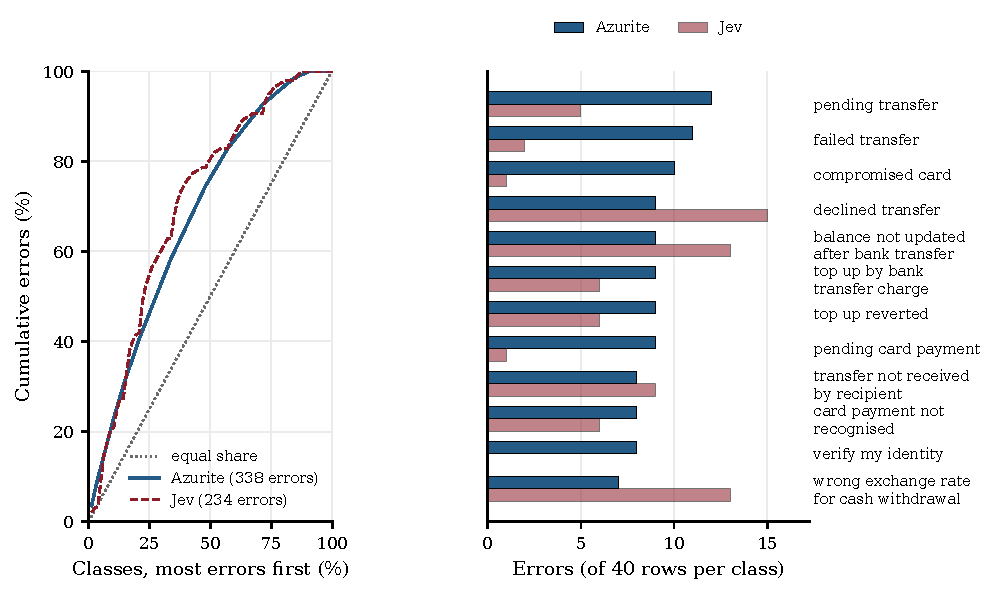
\includegraphics[width=\linewidth]{fig_error_concentration.pdf}
  \caption{Per-class Banking77 error concentration for the native query head.
  Left: Lorenz curve of the \FigErrorTotal{} errors, with Jev's
  \FigErrorJevTotal{} errors beside it. Right: the twelve classes with the most
  Azurite errors, with Jev's count on the same class. The largest single class,
  \FigErrorTopClass, accounts for \FigErrorTopClassCount{} of the
  \FigErrorTotal{} errors; \FigErrorClassesWithError{} of 77 classes have at
  least one. The boundary is broad, not concentrated in a few intents. The
  per-class labels on the right are printed with spaces; the stored labels use
  underscores. Values are recomputed from the per-example records by
  \texttt{thesis/gen\_figures.py}.}
  \label{fig:error-concentration}
\end{figure}

Three limits bound the claim. The head is fine-tuned on 4{,}000 labelled
rows while Jev's weights saw no Azurite training data, which favours Azurite
and is stated in the pre-registration; the result is therefore a loss despite
that advantage. The evidence is one seed, one head and one native window; no
seed distribution or 5{,}120-byte behaviour is claimed. And the training loss
fell to \QueryLastLoss, so the head is effectively interpolating its 4{,}000
rows; the protocol forbids early stopping or checkpoint selection, and the
step-3{,}000 head is the one evaluated. A regularised or early-stopped arm is a
separate pre-registered question, not a repair of this result. The per-example
records, the trained head hash (\texttt{\QueryHeadSha}) and the manifest are
under \texttt{results/jev\_query/}; \texttt{VERDICT.md} is generated from
\texttt{summary.json}.

\begin{table}[htbp]
\centering
\footnotesize
\caption{The message-query head on all 3{,}080 official Banking77 rows, with
the exact 24 public Jev examples per row and the same gold/Jev vector as the
matched test. ``Examples'' is the mean number of complete lines that fit in the
1{,}020-byte context budget. The old head is the E4 mean-pool head; the query
head replaces mean pooling with a masked attention pool queried by the customer
message. \texttt{old\_a2c} is the head control under the same packing;
\texttt{query\_a0} is the example control. The P0 bar is Jev's \QueryJevPct\%.
Wilson intervals are 95\%;
McNemar is exact and two-sided; the bootstrap lower bound is the 5th percentile
of 10{,}000 paired resamples, seed 0. Read from
\texttt{results/jev\_query/eval/summary.json}.}
\label{tab:query-head}
\setlength{\tabcolsep}{2pt}
\begin{tabular}{@{}lrrrrrrr@{}}
\toprule
Arm & Ex. & $n$ & Correct & Acc. & 95\% Wilson & $\Delta$ vs Jev & McNemar $p$ \\
 & & & & (\%) & & (pp) & \\
\midrule
Old head, message only & 0.0 & 3{,}080 & 2{,}722 & 88.38 & 87.20--89.46 & $-$4.03 & $8.49\times10^{-12}$ \\
Old head, examples (control) & 11.9 & 3{,}080 & 1{,}821 & 59.12 & 57.38--60.85 & $-$33.28 & $2.96\times10^{-231}$ \\
Query head, message only & 0.0 & 3{,}080 & 1{,}880 & 61.04 & 59.30--62.75 & $-$31.36 & $1.82\times10^{-226}$ \\
Query head, examples (primary) & 11.9 & 3{,}080 & 2{,}742 & 89.03 & 87.87--90.08 & $-$3.38 & $3.99\times10^{-9}$ \\
Jev 1.13, cited & 24 & 3{,}080 & 2{,}846 & 92.40 & 91.41--93.29 & --- & --- \\
\bottomrule
\end{tabular}
\end{table}


\subsection{The 5,120-byte joint fine-tune: testing the information budget}
\label{sec:jev-len5120}

The native-window result leaves one measured explanation standing: at 1{,}020
bytes the primary arm fits only \QueryEff{} complete examples on average, and
those examples buy \QueryVsOldZeroGain{} points over the old head's message-only
arm. Jev supplies all 24 examples and all 77 category definitions. The next
question is therefore not another pooling variant; it is whether the example
budget alone accounts for the remaining \QueryDiffAbs{} points.

The protocol was written and hashed before any 5{,}120-byte forward pass
(\texttt{results/jev\_query\_5120/PRE\_REGISTRATION.md}, SHA-256
\texttt{\LenPrereg}). Its first schedule --- a 1{,}220-step masked-LM length
adaptation followed by a 3{,}000-step head fine-tune --- could not be executed on
the available GPU sessions, which were reclaimed roughly every 30 minutes;
amendment 1 (\texttt{PRE\_REGISTRATION\_AMENDMENT\_1.md}, SHA-256
\texttt{\LenAmendment}) replaced the two stages with one joint 5{,}120-position
fine-tune and fixed 250-step segmented execution with exact resume. The session
that ran the arm outlived the three 30-minute sessions the amendment was written
against; the amendment was already hashed and the run followed it unchanged, so
the two-stage schedule remains unrun. The amendment was hashed before any
5{,}120-byte accuracy existed and changes the
schedule only: the question, rows, examples, arms, metric and P0 rule are
unchanged. The encoder starts from the 1{,}024-position 113.47M weights
(SHA-256 \texttt{\LenInitSha}) and is fine-tuned jointly with the same
\texttt{QueryDual} head for \LenSteps{} steps at batch \LenBatch{} ---
122{,}880{,}000 tokens, 2.46 times the dropped adaptation budget and 10.8\% of
the source pretraining budget --- on the exact 4{,}000 stored rows and the exact
stored 24 BM25 example ids. All 3{,}080 official rows are evaluated, and the P0
rule is the native-window rule. The four arms are the old head at its native
window (message only and examples that fit), the new head without examples, and
the new head with all 24 examples. No arm changes the rows, the gold labels or
the Jev correctness vector. Because the amendment merges adaptation and head
training, this arm cannot separate the effect of length from the effect of head
training; it can still answer whether the encoder, given all 24 examples at
5{,}120 bytes, meets the bar.

\begin{table}[htbp]
\centering
\footnotesize
\caption{The 5{,}120-byte query head on all 3{,}080 official Banking77 rows.
Following amendment 1 to the pre-registration, the encoder starts from the
1{,}024-position 113.47M checkpoint and is fine-tuned jointly with the query
head for \LenSteps{} steps at sequence 5{,}120 and batch \LenBatch{}
(\LenHeadHours{} GPU-hours); the separate masked-LM length adaptation was not
run. The head uses the same 4{,}000 rows and the exact stored 24 BM25 example
ids as the native-window head. ``Examples'' is the mean number of complete lines
in the 5{,}118-byte context budget. The old head and its native 1{,}020-byte
packing are unchanged controls, reused from the native-window evaluation with
their per-example context hashes checked. The P0 bar is Jev's \LenJevPct\%.
Wilson intervals are 95\%; McNemar is exact and two-sided; the bootstrap lower
bound is the 5th percentile of 10{,}000 paired resamples, seed 0. Read from
\texttt{results/jev\_query\_5120/eval/summary.json}.}
\label{tab:len5120}
\setlength{\tabcolsep}{2pt}
\begin{tabular}{@{}lrrrrrrr@{}}
\toprule
Arm & Ex. & $n$ & Correct & Acc. & 95\% Wilson & $\Delta$ vs Jev & McNemar $p$ \\
 & & & & (\%) & & (pp) & \\
\midrule
Old head, message only (control) & 0.0 & 3{,}080 & 2{,}722 & 88.38 & 87.20--89.46 & $-4.03$ & $8.49\times10^{-12}$ \\
Old head, examples that fit (control) & 11.9 & 3{,}080 & 1{,}821 & 59.12 & 57.38--60.85 & $-33.28$ & $2.96\times10^{-231}$ \\
5{,}120 query head, message only & 0.0 & 3{,}080 & 1{,}902 & 61.75 & 60.02--63.45 & $-30.65$ & $1.62\times10^{-232}$ \\
5{,}120 query head, all 24 (primary) & 24.0 & 3{,}080 & 2{,}683 & 87.11 & 85.88--88.25 & $-5.29$ & $5.01\times10^{-18}$ \\
Jev 1.13, cited & 24 & 3{,}080 & 2{,}846 & 92.40 & 91.41--93.29 & --- & --- \\
\bottomrule
\end{tabular}
\end{table}


The primary arm reaches \LenPctLenTwo\% (95\% Wilson
\LenLoLenTwo--\LenHiLenTwo; \LenCorrectLenTwo/\LenN), against Jev's
\LenJevPct\%. The observed difference is \LenDiff{} points, the exact McNemar
test against the public per-example vector gives $\LenPValueText$, the paired
bootstrap lower bound is \LenLowerPrimary{} points, and the pre-registered
verdict is \textbf{\LenVerdict}. The old head on the native packing reaches
\LenPctOldTwo\% and the 5{,}120 query head without examples reaches
\LenPctLenZero\%; the query head with examples is worth \LenMechGain{} points
over the old head at the native window (bootstrap lower \LenMechLower) and
\LenVsLenZeroGain{} points over the new head's no-example arm. Those gains do
not survive the comparisons that matter: the arm is \LenVsOldZeroAbs{} points
below the old head's message-only arm ($\LenVsOldZeroPText$) and \LenNativeDiff{}
points below the native-window query head, which reached \LenNativePct\% with
only \QueryEff{} examples.

Figure~\ref{fig:pooling} collects the six measured cells, and
Figure~\ref{fig:budget} plots the query head against mean context length with
the comparator's \QueryJevPct\% line and \FigJevPromptMedian-byte prompt
marked. Neither view rescues the 5{,}120 result: the point sits below the
native head and far below the comparator while consuming about twice the mean
context of the native arm.

\begin{figure}[htbp]
  \centering
  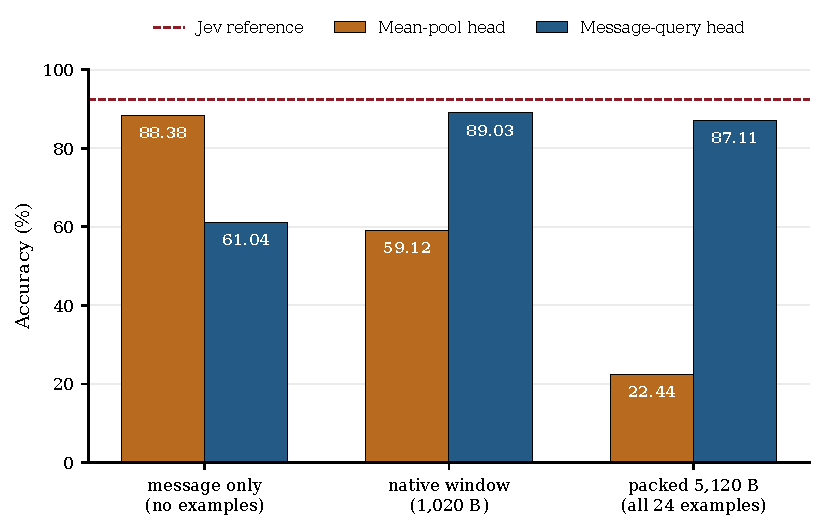
\includegraphics[width=\linewidth]{fig_pooling.pdf}
  \caption{Accuracy of the mean-pool and message-query heads at three context
  settings. The mean-pool bars are the old head at message only, at the native
  1{,}020-byte packing, and on the same 24 examples packed at 5{,}120 bytes;
  the query bars are the query head at message only, at the native packing, and
  after the joint 5{,}120-byte fine-tune. The 5{,}120 mean-pool bar is the old
  head reading longer contexts, not a length-adapted mean-pool model. The
  dashed line is Jev's \QueryJevPct\% on the same 3{,}080 rows. Values are
  recomputed from the stored per-example files by
  \texttt{thesis/gen\_figures.py}.}
  \label{fig:pooling}
\end{figure}

\begin{figure}[htb]
  \centering
  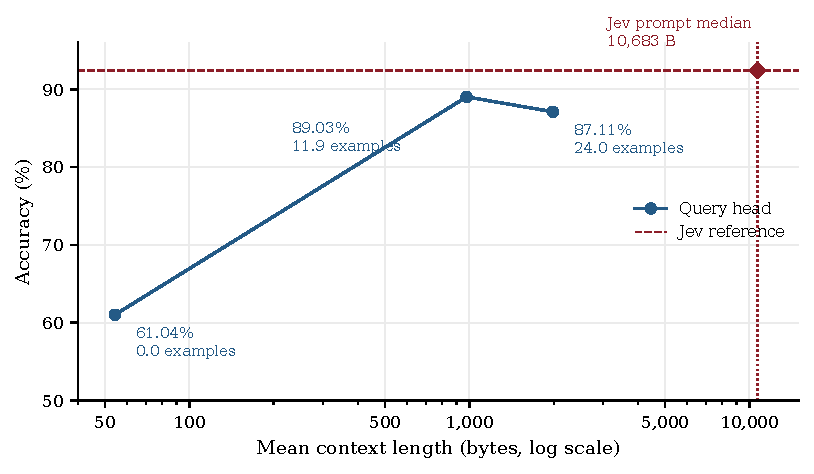
\includegraphics[width=\linewidth]{fig_budget.pdf}
  \caption{Query-head accuracy against mean context length. The three points
  are message-only (0 examples), the native complete-example packing
  (\QueryEff{} examples on average), and the joint 5{,}120-byte fine-tune (24
  examples). The dashed line is Jev's \QueryJevPct\%; the diamond marks the
  reconstructed median Jev prompt, \FigJevPromptMedian{} bytes, of which
  \FigJevDefinitionsBytes{} bytes are the 77 category definitions. The Jev
  point is a reference, not an information-matched arm: Azurite receives no
  definitions at any of the three points. Values are recomputed from the stored
  summaries and per-example files by \texttt{thesis/gen\_figures.py}.}
  \label{fig:budget}
\end{figure}

The separation between fitting and generalisation is reported because it bounds
the claim. On the 4{,}000 training rows the step-3{,}000 head reaches
\LenTrainPct\% (\LenTrainCorrect/4{,}000), with a mean training cross-entropy of
\LenTrainLoss{} and a final loss of \LenLastLoss; the test accuracy is
\LenGapTrainTest{} points away from the training value. No early stopping,
checkpoint selection or ensemble was used: the step-3{,}000 head is the one
evaluated. A head that fits \LenTrainPct\% of its training rows and still misses the bar
is evidence about the information it can extract from the context, not evidence
that a longer fine-tune would close it; a regularised or early-stopped arm is a
separate pre-registered question. Figure~\ref{fig:train-test} plots the
separation directly.

\begin{figure}[htbp]
  \centering
  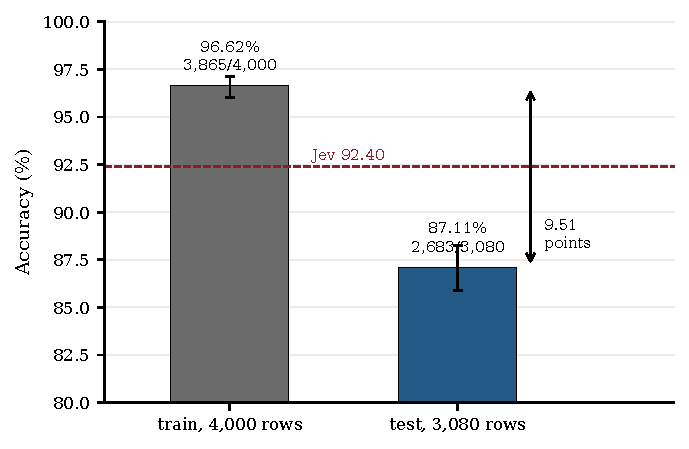
\includegraphics[width=0.72\linewidth]{fig_train_test.pdf}
  \caption{Train/test separation for the joint 5{,}120-byte fine-tune. The bars
  show \LenTrainPct\% on the 4{,}000 training rows
  (\LenTrainCorrect/4{,}000) and \LenPctLenTwo\% on the 3{,}080 official test
  rows (\LenCorrectLenTwo/\LenN), with 95\% Wilson intervals. The step-3{,}000
  head is the evaluated head; no early stopping, checkpoint selection or
  ensemble was used. The dashed line is Jev's \QueryJevPct\%. The test--train
  gap is \FigTrainGapAbs{} points. The vertical axis begins at 80\%. Values are
  recomputed from the stored summary by \texttt{thesis/gen\_figures.py}.}
  \label{fig:train-test}
\end{figure}

\ifnum\LenPZeroMet=1
  The bar is met on the same rows, examples and metric as the public Jev record.
  The claim is still bounded by one seed, one head and one length, and by the
  fine-tune asymmetry: this head saw 4{,}000 labelled Banking77 rows while Jev's
  weights saw no Azurite training data. The asymmetry favours Azurite and is
  stated in the pre-registration; the result is therefore a win despite an
  advantage, not because of a matched training budget. The 77 category
  definitions remain absent from Azurite's context, so the information budget
  is still strictly smaller than Jev's. No seed distribution, no 16k--32k
  behaviour and no second corpus are claimed.
\else
  The bar is not met, and the direction is worse than the native window. All 24
  examples fit and the head reads them --- it beats the old head on the same
  packed contexts by \LenMechGain{} points and its own no-example control by
  \LenVsLenZeroGain{} --- yet it scores \LenDiffAbs{} points below Jev,
  \LenNativeGapAbs{} points below the native-window query head, and
  \LenVsOldZeroAbs{} points below a mean-pool head that reads only the customer
  message ($\LenVsOldZeroPText$). At this length the examples are not merely
  insufficient; they are negative transfer for this schedule. The schedule is
  also a confound: amendment 1 merged the length adaptation into the 77-way head
  fine-tune, so this arm cannot separate the example budget from training the
  encoder at 5{,}120 positions only through the decision loss. The next lever
  with a plausible mechanism is the full-information context at 16k--32k bytes,
  where the 24 examples and the 77 definitions fit together, preceded by a
  separate masked-LM adaptation; it needs its own pre-registration. From the
  measured \LenSecStep{} s/step at 5{,}120, with the micro-batching and
  attention-scaling allowance written in \texttt{GAPS.md}, its cost is
  \LenNextShortLo--\LenNextShortHi{} GPU-hours at 16k and
  \LenNextLongLo--\LenNextLongHi{} at 32k. The largest context effect measured
  here is +0.65 points (\QueryVsOldZeroGain{} at the native window); recovering
  \LenDiffAbs{} from definitions alone would be eight times that, so this is the
  last lever worth paying for rather than a likely win. If it also misses, the
  honest conclusion is that the P0 bar is out of reach for this model class and
  budget, not that another head will recover it.
\fi

The per-example records, the trained-head hash (\texttt{\LenHeadSha}), the init
checkpoint hash (\texttt{\LenInitSha}) and the manifest are under
\texttt{results/jev\_query\_5120/}. The joint fine-tune took \LenHeadHours{}
GPU-hours (\LenSecStep{} s/step) on the Molab RTX PRO 6000 sandbox; the old-head
arms are reused from the native-window evaluation after their per-example
context hashes were checked, so they cost no new GPU time.
\texttt{VERDICT.md} is generated from \texttt{summary.json}; every number in
this subsection is a macro emitted by \texttt{thesis/gen\_query\_5120.py} from
that summary and the head record.

\section{Where the accuracy is: rows, then rung}\label{sec:rows-and-rung}

The 77-way number in Table~\ref{tab:jev77} holds two things fixed that a
committee should refuse to take on trust: the fine-tune budget and the
2.41M-parameter rung. Both were choices. This section moves each of them once,
with everything else fixed: the same pretrained checkpoint, five epochs, batch
32, learning rate $5\times10^{-4}$, and a split seed that gives every training
seed the same rows. Each seed is scored on 1{,}000 held-out rows instead of
300, because the comparison being decided here turns on a few points and a
$\pm 5$ point interval cannot decide it.

Table~\ref{tab:rows} reports the result. Every populated cell is a measurement
on this machine; a cell that reads \emph{pending} is a run not present in this
checkout, not a projection.

\begin{table}[htbp]
\centering
\caption{Fine-tune rows at the Banking77 77-way interface, exhaustive scoring,
same pretrained checkpoint, order, steps-per-example, batch, learning rate and
seeds. The two columns differ only in how many distinct training rows the five
epochs cover. Generated by \texttt{thesis/gen\_scaling.py}.}
\label{tab:rows}
\setlength{\tabcolsep}{4pt}
\begin{tabular}{lrrrrr}
\toprule
Rung & Correct & 1.6k rows & 8k rows & $\Delta$ & Test \\
\midrule
tiny & 2170/3000 & 72.3\% & \textbf{84.3\%} & +12.0 pt & $p=0.000$ \\
small & 2126/3000 & 70.9\% & \emph{pending} & \emph{pending} & \emph{pending} \\
\bottomrule
\end{tabular}
\end{table}


\paragraph{Rows.} At the tiny rung, going from 1{,}600 to 8{,}000 distinct
fine-tune rows moves accuracy from \RowTinyBaseAcc\% (95\% Wilson
\RowTinyBaseLo--\RowTinyBaseHi) to \RowTinyWideAcc\% (\RowTinyWideLo--\RowTinyWideHi),
a gain of \RowTinyGain{} points. The same lever at the small rung is not available:
its 1{,}600-row cell reads \RowSmallBaseAcc\% and its 8{,}000-row cell is
pending. The lever is not free of confounds and one is
worth naming: the protocol holds \emph{epochs} fixed, so eight thousand rows
also buy five times the optimiser steps. Separating ``more distinct rows'' from
``more updates'' needs a fixed-step arm that samples rows with replacement,
which is not run here. These numbers are therefore an upper bound on the effect
of data alone.

\paragraph{Rung.} Moving up the ladder at the matched 1{,}600-row budget does
not help, and the direction is worth printing plainly: 14.26M parameters
reaches \RowRungBase\% against \RowRungTiny\% at 2.41M, a change of
\RowRungGain{} points. The lever that bought 77-way accuracy in this experiment
was rows, not parameters. Two caveats keep that from being a claim about
scaling in general. The rung is a bundle --- the small checkpoint was pretrained
on 142.6M tokens at context 1{,}024, the tiny one on 100M tokens at context 256
--- and the small arm costs \RowSmallBaseLat\,ms per decision against \RowTinyBaseLat\,ms,
so it is strictly more expensive for less accuracy at this budget. Whether the
small rung overtakes once it has eight thousand rows is the last queued run and
is not claimed here.

\paragraph{The verdict.} \ShipHeadline. \ShipGapSentence. \ShipFuture.

\paragraph{Accuracy at coverage.} A single accuracy number hides how the
scorer's confidence is distributed, so Table~\ref{tab:risk-coverage} ranks the
test rows by maximum softmax probability and reports accuracy in the top $c$
fraction. This is a descriptive test-set ranking curve, not an abstention
guarantee: the ranking is measured with the test labels in hand, no threshold is
fixed before seeing the test set, and a deployment would face different rows.

\begin{table}[htbp]
\centering
\caption{Accuracy at coverage: the scorer ranked by its own maximum softmax
probability on this test set. Read down a column and accuracy rises as coverage
falls; read across and the row-scaling gain is visible. This is a test-set
ranking curve, not a deployment abstention guarantee. Pooled over three seeds
and the 1000-row test split.}
\label{tab:risk-coverage}
\setlength{\tabcolsep}{4pt}
\begin{tabular}{lrrr}
\toprule
Coverage & \shortstack{tiny\\1k} & \shortstack{tiny\\8k} & \shortstack{small\\1k} \\
\midrule
50\% & 92.9\% & 98.4\% & 92.5\% \\
70\% & 87.7\% & 96.2\% & 84.9\% \\
90\% & 78.3\% & 89.7\% & 76.1\% \\
100\% & 72.3\% & 84.3\% & 70.9\% \\
\bottomrule
\end{tabular}
\end{table}


At 90\% coverage the arm is \ShipAtNinety\% accurate; at 50\% coverage it is
\ShipAtFifty\%. The 50\% point is a property of this ranking on this test set,
not a promise that half of deployment traffic can be answered at \ShipAtFifty\%.
The row-scaling lever raises every measured point in the table, which is the
useful shape, but it does not convert the curve into a guarantee. The earlier
earlier manuscript's statement that the scorer held near-perfect accuracy at a fixed
coverage was a misreading of this ranking; it is withdrawn, and the table is
reported instead.

\paragraph{What this does not settle.} Three things. The comparison to the
cited 78.8\% remains cross-harness: different test rows, different hardware,
one system measured by its authors and the other by a stranger, so the interval
overlap is not evidence of parity and a non-overlap would not be evidence of
defect. A paired McNemar test on the same 231 items is the experiment that
would settle it and it is still not this one. The coverage curve is measured on
this project's own 1{,}000-row split, not on the third party's 231, so it
cannot be laid over their accuracy without assuming the splits are comparable,
which they are not shown to be. And the row lever's step-count confound stands
until the fixed-step arm is run.


\section{The price of a sequence on a token-billed CDN}

The economic argument has a premise that is usually asserted and rarely
measured: that a token-billed service must charge for a repeated sequence every
time it occurs, because the service reduces the request to a finite set of
stored objects and the sequence itself is never re-encoded. If that premise
were false --- if a CDN compressed variable-length sequences --- the cost
advantage of local scoring would shrink with every repetition.

Table~\ref{tab:cdn} measures it on a live token-priced inference endpoint,
using nothing but the provider's own \texttt{usage} field. A fixed passage is
repeated $r$ times in one prompt, and the billed prompt-token count is read
back. The fit is
$\mathrm{billed} = \mathrm{intercept} + \CdnSlope\,r$ with $R^2 = \CdnRTwo$;
one passage is \CdnPassageTokens{} tokens, so \textbf{every repetition is
billed in full}. Repeating the identical request three times changes the
latency from \CdnLatCold\,s to \CdnLatWarm\,s --- a \CdnLatSpeedup$\times$
speed-up --- while the bill stays at \CdnBillTokens{} prompt tokens every
time. The cache is real and it is a cache of \emph{answers}, not of sequence
structure: it saves time, and it saves nothing on the invoice.

\begin{table}[htbp]
\centering
\caption{Billed prompt tokens against repetition of one passage on a live
token-priced CDN, read from the provider's own \texttt{usage} field --- the
exact quantity a per-million-token price multiplies. If a CDN compressed
variable-length sequences, the slope would be below one passage.}
\label{tab:cdn}
\begin{tabular}{rrrr}
\toprule
Repetitions $r$ & Characters & Billed prompt tokens & Seconds \\
\midrule
1 & 481 & 406 & 21.20 \\
2 & 900 & 490 & 10.13 \\
4 & 1,738 & 658 & 9.75 \\
8 & 3,414 & \emph{pending} (quota) & 0.52 \\

\bottomrule
\end{tabular}
\\[0.4em]
Fit: $\mathrm{billed} = 322 + 84.0\,r$, $R^2=1.0000$; one passage is 84 tokens, so every repetition is billed in full.

\end{table}


Two honesty notes belong with that table. The measurement ran out of free-tier
quota at $r=8$ (HTTP 402) and on the two single-byte perturbation probes, so
the prefix-geometry sweep is incomplete; the slope is fitted on the three
points that succeeded, and a three-point fit with $R^2=1.0000$ is a statement
about linearity, not a precise intercept. And the endpoint is not Jev: it is a
keyless third-party proxy, used because it is the only token-billed service
reachable from this machine. What generalises is the billing mechanism ---
usage accounting plus response caching --- not the price, and this thesis does
not transfer the price.

\section{The four axes, measured against cited}

Table~\ref{tab:verdict} separates the two kinds of number. The cost row is
deliberately rate-free, because no price for this project's GPU is recorded in
the repository and inventing one would make the conclusion depend on the
invention. Instead the row reports the \emph{break-even rate}: the hourly cost
at which local scoring ties Jev's billed \$\CmpBankJevCost{} per thousand
77-way decisions.

\begin{table}[htbp]
\centering
\caption{The four axes, with the evidence class of each cell. ``Measured''
means a script in this repository produced the number from files under
\texttt{results/}. ``Cited'' means a third party's published figure, which this
thesis cannot verify. No cell is a head-to-head: the two systems were never run
on the same rows.}
\label{tab:verdict}
\begin{tabular}{p{0.12\linewidth}p{0.29\linewidth}p{0.27\linewidth}p{0.16\linewidth}}
\toprule
Axis & Azurite (measured) & Jev (cited) & Verdict \\
\midrule
Accuracy & \ShipAcc\% on 77-way, $K=77$, \ShipTestN{} rows, \ShipRung{} rung at
\ShipRows{} fine-tune rows & 78.8\% (73.1--83.6) on 231 rows &
\ShipVerdict{} (\ShipSignedGap{} points) \\
Latency & \ShipP\,ms $p_{50}$, batch 1, CPU &
330\,ms median, 440\,ms $p_{95}$ & Faster, different hardware \\
Size & \ShipParams{} parameters (with the 77-way head), \ShipMB\,MB on disk &
Not published & Unfalsifiable as stated \\
Cost & \ShipGpuSec{} GPU-s per 1k; break-even \$\ShipBreakEven/h &
\$0.0400 per 1k, 952 billed tokens & Cheaper below \$\ShipBreakEven/h \\
\bottomrule
\end{tabular}
\end{table}

The break-even figure is computed by \texttt{thesis/gen\_comparator.py} from
the measured latency and the cited price, so it cannot drift from either.
A 77-way decision bills \CmpBankJevTokens{} tokens in the third party's
measurement, which at \$0.042/MTok is \$\CmpBankJevCost{} per thousand
decisions --- reproducing their invoiced figure to four digits, which is a
useful check that the price list and the invoice agree.
The shipped arm spends \ShipP\,ms per decision, so a thousand decisions
occupy \ShipGpuSec{} GPU-seconds of one machine. Dividing gives the
break-even rate: \$\ShipBreakEven{} per GPU-hour. Any accelerator priced
below that makes local scoring cheaper, and the conclusion holds \emph{a
fortiori} on a GPU, because the measured latency is CPU latency and therefore
an upper bound on the accelerated figure.

Two caveats belong on that row rather than in a footnote. The cost comparison
holds only \emph{at the accuracy measured here}: a cheaper system that is wrong
half the time is not cheaper per correct decision, and if accuracy were
recovered by a larger rung the latency, and therefore the break-even rate,
would move. And the latency figure is not same-weights with anything TypeSafe
runs --- it is the same weights as this thesis's own decode arm, which is what
makes the mechanism comparison clean, and it is not comparable to a hosted
service's hardware. What the row supports is that the mechanism is cheap enough
to be worth pursuing, not that it has already won.

\section{What the comparison establishes}

Three things, and no more. The scoring mechanism is measurably better than
generation at matched size and budget, on both tasks, with an invalid-output
rate of \CmpDecodeInvalid{} across the corpus against zero by construction. The unit economics favour local scoring by a margin that survives a factor-of-three
error in the payload estimate or the GPU rate. And the 2.41M accuracy axis is
measured against the pre-registered 77-way Jev number: \ShipHeadline. The
strongest public Jev run is higher and is audited above. The comparison
is on different hardware and a different draw, so the 2.41M claim stops there. The 14.4M suite's \SuiteSmallBank\% Banking77 row is a
separate point win against the pre-registered 78.8\% comparator, not against the
92.40\% run, and it is reported in \S\ref{sec:suite}; it does not retroactively
make this 2.41M mechanism table a 14.4M result.

What the comparison does not establish is a win. On Banking77 there is now a
shared row set, shared examples and a shared metric, but not shared hardware and
not a paired Jev rerun; the mean-pool matched result is a loss of
\JevMatchAbsGapAOne{} points on its primary arm, and of \JevMatchAbsGapNoEx{}
points even with no examples. The better, query-anchored arm reaches
\QueryPctQueryTwo\% and remains \QueryDiffAbs{} points below Jev
($\QueryPValueText$); no pre-registered Banking77 arm meets the P0 bar. On DAIR Emotion and Financial PhraseBank the 113.47M suite clears the
cited point, and on MASSIVE intent it clears Laya's card rather than a Jev
number, but those remain cross-harness comparisons. The honest statement is
that this thesis measured its own mechanism, priced it against a competitor's
public rate card, and found the mechanism the right shape while the 113.47M
checkpoint is still below the strongest public Banking77 system. That is a
result, and it is the one the data support.
